\section{数値解析例}
本節では,Na型モンモリロナイトに対する水和エネルギーを用いて行ったCG-MD
シミュレーションの結果を示す.
CG-MD解析では,温度,相対湿度,圧力を一定に保った状態で非平衡状態にある
初期モデルから,モンモリロナイト含水系(以下,粘土含水系と呼ぶ)の
CG-MDモデルで緩和計算を行う.
これを6つの異なる相対湿度において行い,膨潤挙動の観点からみたときの,
シミュレーション結果の妥当性について議論する.
以下,初期モデルと計算手順を述べた後,シミュレーション結果を
粘土分子配置のスナップショットと層間距離の頻度分布を示す。
これらの結果をもとに,相対湿度に応じた膨潤状態の変化について述べる.
\subsection{初期モデルの作成}
緩和計算を行うための初期モデルを図\ref{fig:fig3}-(a)に示す.
これは2021年度の共同研究報告書で述べた方法で作成した粘土含水系モデルの一つで,
粗視化粒子数3,194で構成された,80の粘土分子からなる.
このモデルは以下の手順で作成されている.\\
はじめに,直線状の粘土分子を200$\times$200[nm$^2$]の
矩形領域に互いに重ならないように,位置と向きをランダムに配置する.
この矩形領域を周期構造を構成する単位セルとして,
乾燥密度が約1.6g/cm$^{3}$となるまで1[ns]かけて断熱圧縮する.
その際,粒子系の運動方程式を時間積分するための時間ステップ幅
は0.02[ps],時間ステップ数は5万ステップとしており,
時間積分に関するこの条件は以後の解析でも同じである.
断熱圧縮過程では系の温度を制御していないため,圧縮によって系
に加えれられたエネルギーによって高温になり平衡状態にも無い.
そこで,圧縮後のモデルを300Kまで$250$psをかけて冷却し,
その後750psの間一定温度(300K)で緩和計算を行う.
なお,ここでいう緩和とは,温度や体積などの外的条件を一定にして,
系を平衡状態に向けて推移させることを意味する.
以上の計算では,各粗視化粒子において水分量を表す
パラメータである粒子間相互作用ポテンシャルの特性距離$\sigma$を,
二層膨潤状態に相当する$\sigma=1.5$[nm]に固定し,
系内での水分移動も系外との水分の授受もないものとしている.
最後に,無次元化された化学ポテンシャル$\bar \mu$を$0.5$に保ち,
温度,体積一定のもと,水分分布を含めた緩和計算を1[ns]間行う.
このとき,$\bar \mu$の値は強い排水が起こるように設定されており,
緩和計算後,大きな層外空隙をもつ組織構造が得られる.\\
図\ref{fig:fig3}-(a)は以上の手続きによって得た粘土含水系モデルである.
本年度の研究では,これを初期構造とし,Na型モンモリロナイトの
水和エネルギーモデルを用いて,相対湿度に応じてどのような組織構造
へ移行するか調べる.
初期構造を得るまでの計算では,昨年度の研究で検討を行った
水和エネルギーモデルの一つである振動モデルを用いている.
このモデルは仮想的な粘土の水和挙動を表現したものであるため,
図\ref{fig:fig3}-(a)の状態は,今回新たに作成した水和エネルギーモデル
の下では平衡状態にない.そのため,相対湿度の設定値によらず,
水分や分子配置には必ず何らかの変化が生じる.
\subsection{相対湿度50$\%$に対する結果}
図\ref{fig:fig3}の(b)と(c)は,相対湿度50$\%$,温度300K, 圧力10MPaで
1ns間,緩和計算を行ったときの粘土含水系の変化を示したものである.
(b)は経過時間が250psの時点での分子配置を,(c)は1nsの時点で緩和計算
を終了した最終的な結果を示している.
(a)と(b)の図から明らかなように,初期状態では非常に水分量が少ないため,
緩和計算の初期の段階で速やかに吸水がおき,積層間隔が拡がるとともに,
図中A-Dのラベルで示した層外間隙の量が明らかに減少している.
一方,(b)から(c)の間では,粘土分子の配置にあまり変化がなく安定した構造が
形成されていると考えられる.
特に,間隙AやBは収縮量が大きくAはほぼ消失している.これに対して,
粘土分子を巻き込むことで形成された層外間隙CとDは,吸水によって
粘土層間の拡張に伴う収縮量は小さく,水分量の変化に対し組織構造を
維持する役割を果たしていると推察される.
なお,ここでは領域の体積は拘束されていないため,(a)から(b)と(c)へ
推移する仮定で若干の体積収縮が認められる.
このように,吸水による層間距離の拡張がある場合も,系全体としては
収縮が起きることもあり得ることは,マクロスコピックな意味での
膨潤挙動について考える際にも留意する必要があることを示唆している.
%--------------------
\begin{figure}[h]
	\begin{center}
	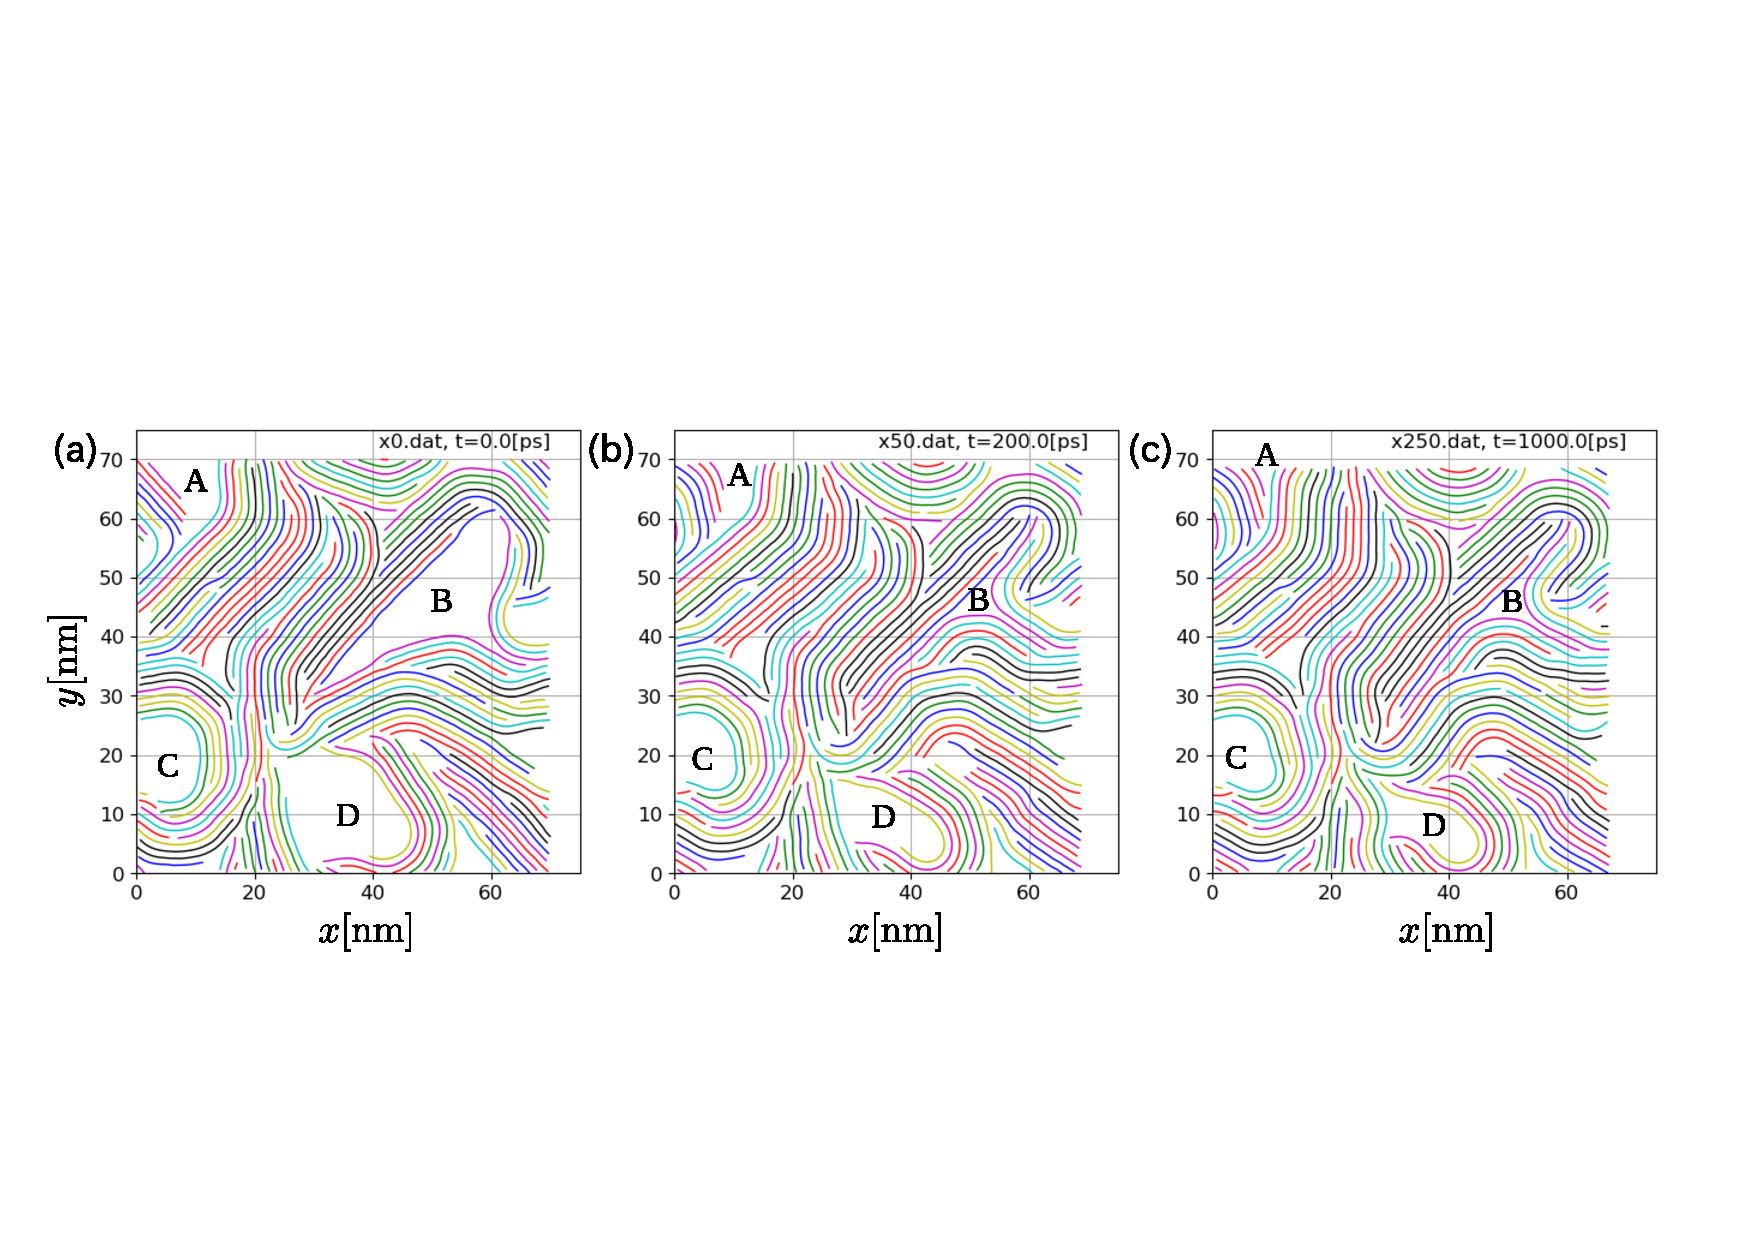
\includegraphics[width=1.0\linewidth]{Figs/fig3.pdf} 
	\end{center}
	\caption{
		相対湿度50$\%$での緩和にともなう粘土分子配置の変化.  
		(a)は初期状態,(b)緩和開始から200psの状態,(c)は1ns経過後の最終状態.
		A-Dのラベルは粘土層外の主要な空隙を示す.
	} 
	\label{fig:fig3}
\end{figure}
\subsection{相対湿度による組織構造の違い}
相対湿度50$\%$の場合に加えて,10,20,65,75および90$\%$で同様にして
緩和計算を行った結果を図\ref{fig:fi4}に示す.
相対湿度以外の計算条件は前項50$\%$の場合と同じである.\\
これらの結果のうち,相対湿度が最も低い(a)10$\%$のケースでは,
初期構造からあまり変化が見られず,層外間隙の形や大きさは
当初の状態と同程度のままになっている.これは,初期構造が
相対湿度が極めて低い場合に生じうるものであったことを意味する.
ただし,系全体の体積はやや収縮しており,若干の排水が起きている
ものと予想される.この次に低い湿度の(b)20$\%$では,全体の体積は
(a)と同程度の収縮となっているが,層外間隙は収縮が大きいものも
あり,相対湿度50$\%$によく似た分子配置となっている.
ただし(c)のケースよりも初期状態からの系全体の収縮量は
(b)の方が大きく,(b)から(c)の相対湿度範囲で排水から吸水が
進行し始めるものと解釈できる.
これに対して(d)の65$\%$の場合,全体体積の変化はほぼ無視できる
程度である一方,層間距離は(c)の場合よりも広く,明らかに吸水
に転じていることが分かる.この段階では,粘土分子の巻き込み
で残留した空隙もかなりの程度圧縮が進んでいる.
さらに相対湿度の高い(e)と(f)では,系全体としても膨張する
様子が見られ,このことは,層外間隙の体積収縮が(d)のとき
以上には進行していないことと呼応している.
%--------------------
\begin{figure}[h]
	\begin{center}
	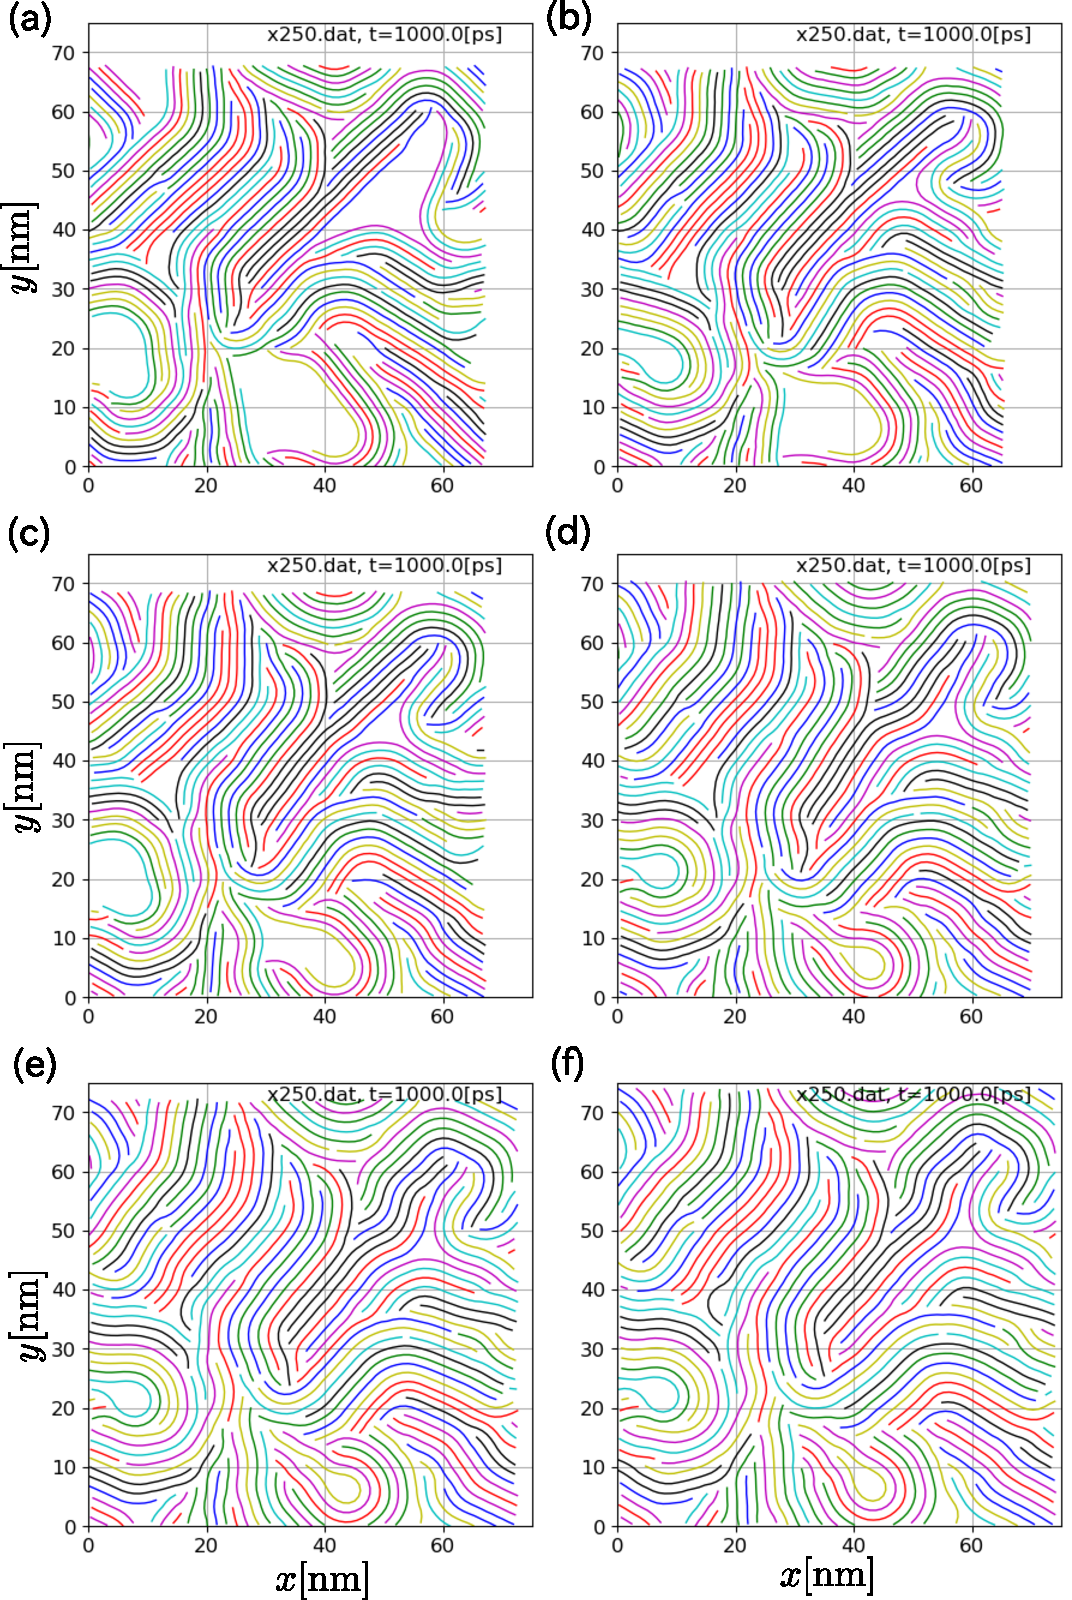
\includegraphics[width=0.8\linewidth]{Figs/fig4.pdf} 
	\end{center}
	\caption{
		6つの異なる相対湿度において得られた粘土含水系の組織構造.
		相対湿度は,(a)から(f)の順に10,20,50,65,75および90$\%$. 
		相対湿度50$\%$の結果は,図\ref{fig:fig3}-(c)と同じものを再掲.
	} 
	\label{fig:fig4}
\end{figure}
\subsection{追加したテキスト}
図2
湿度を指定して行った,Na型モンモリロナイトの膨潤シミュレーション.(a)は粘土含水系モデルの初期状態を,(b)は相対湿度50$\%$, 
(c)は 相対湿度75$\%$において緩和計算を行い最終的に得られた組織構造(粘土分子配置)のスナップショットを示す.

(a)に示した初期状態は2021年度共同研究で得られた,仮想的な粘土の組織構造モデルである.
このモデルでは系全体が一層膨潤に達するには不十分な水分量しかもたない,乾燥状態に近いモデルになっている.
これを始状態とし,相対湿度をそれぞれ50$\%$および75$\%$に設定し,温度を300で一定として組織構造の緩和(平衡化)
計算を行った結果が(b)と(c)である.いずれもの場合も吸水が起こり,粘土層間距離が拡がっている.
その結果,粘土分子の積層体は顕著に体積が増す一方,粘土層外の間隙が積層体の体積増加を吸収するためにモデル全体の膨潤量は小さい.
湿度75$\%$のケースでは50$\%$に比較して吸水量が大きく,積層体の体積膨張もより大きいため,層外の間隙がほとんど消失していることが分かる.

図3
湿度を指定して行ったNa型モンモリロナイトの膨潤シミュレーションの結果.
(a)は初期状態,(b)は相対湿度50$\%$, (c)は 相対湿度75$\%$における粘土層間距離の頻度分布を示す.

初期状態(a)では層間距離が11〜12Åの範囲にあり0層から1層膨潤状態への中間にある.
この状態から相対湿度を50$\%$にして緩和計算を行った結果である(b)では,層間距離は12.5Å近傍に集中し,
ほぼ1膨潤状態のみとなっている.さらに相対湿度をあげた75$\%$では,13.2$\AA$と15.5$\AA$付近に2つのピークを持つ頻度分布となっている.
頻度分布の前者のピークは,1層から2層膨潤へ移行する直前の,後者のピークは2層膨潤状態の層間距離に相当し,
このケースでは1層と2層膨潤状態が混在することを示している.
いずれの相対湿度も,図1-(a)に示したXRD試験で観測される層間距離と近い値であることがわかる.
このことからも,本研究で用いた水和エネルギーモデルには,観測で得られたNa型モンモリロナイトの膨潤特性が反映されていることが確かめられる.
%--------------------
\begin{figure}[h]
	\begin{center}
	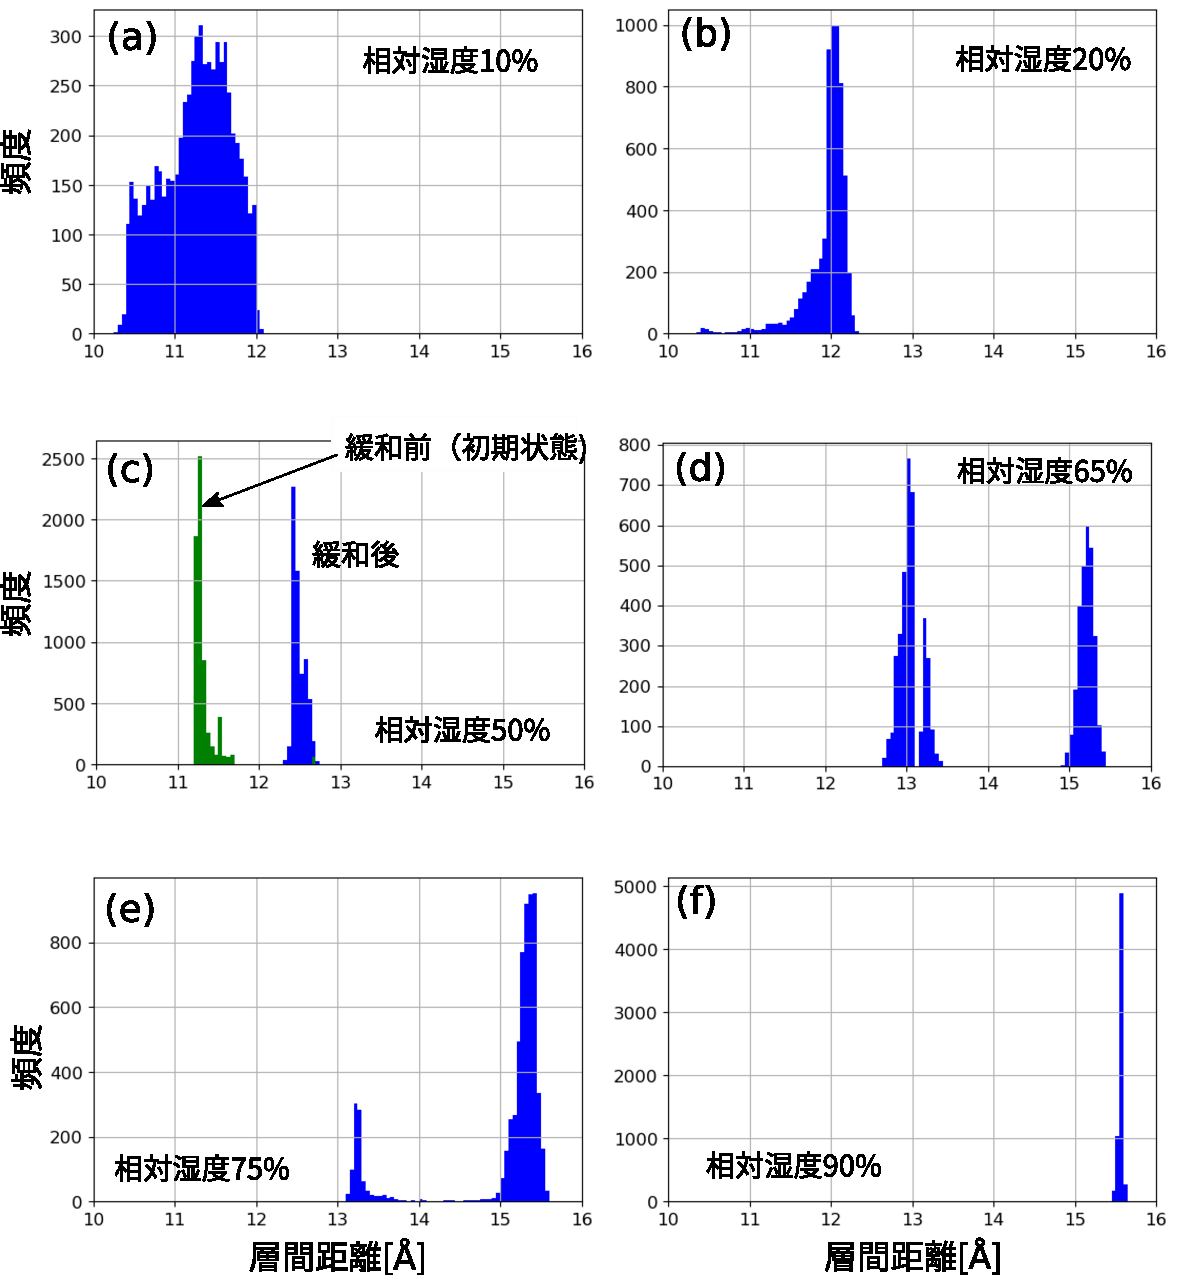
\includegraphics[width=1.0\linewidth]{Figs/fig5.pdf} 
	\end{center}
	\caption{
		caption.
	} 
	\label{fig:fig5}
\end{figure}
%--------------------
